%%%%%%%% ICML 2022 EXAMPLE LATEX SUBMISSION FILE %%%%%%%%%%%%%%%%%

\documentclass[nohyperref]{article}

% Recommended, but optional, packages for figures and better typesetting:
\usepackage{microtype}
\usepackage{graphicx}
\usepackage{subcaption}
\usepackage{booktabs} % for professional tables

% hyperref makes hyperlinks in the resulting PDF.
% If your build breaks (sometimes temporarily if a hyperlink spans a page)
% please comment out the following usepackage line and replace
% \usepackage{icml2022} with \usepackage[nohyperref]{icml2022} above.
\usepackage{hyperref}


% Attempt to make hyperref and algorithmic work together better:
\newcommand{\theHalgorithm}{\arabic{algorithm}}

% Use the following line for the initial blind version submitted for review:
% \usepackage{icml2022}

% If accepted, instead use the following line for the camera-ready submission: 
\usepackage[accepted]{icml2022}

% For theorems and such
\usepackage{amsmath}
\usepackage{amssymb}
\usepackage{mathtools}
\usepackage{amsthm}

% if you use cleveref..
\usepackage[capitalize,noabbrev]{cleveref}

%%%%%%%%%%%%%%%%%%%%%%%%%%%%%%%%
% THEOREMS
%%%%%%%%%%%%%%%%%%%%%%%%%%%%%%%%
\theoremstyle{plain}
\newtheorem{theorem}{Theorem}[section]
\newtheorem{proposition}[theorem]{Proposition}
\newtheorem{lemma}[theorem]{Lemma}
\newtheorem{corollary}[theorem]{Corollary}
\theoremstyle{definition}
\newtheorem{definition}[theorem]{Definition}
\newtheorem{assumption}[theorem]{Assumption}
\theoremstyle{remark}
\newtheorem{remark}[theorem]{Remark}

% Todonotes is useful during development; simply uncomment the next line
%    and comment out the line below the next line to turn off comments
%\usepackage[disable,textsize=tiny]{todonotes}
\usepackage[textsize=tiny]{todonotes}


% The \icmltitle you define below is probably too long as a header.
% Therefore, a short form for the running title is supplied here:
\icmltitlerunning{One Datapoint is Not Enough: Disentangling Grouped Data with Confounding}

\begin{document}

\twocolumn[
\icmltitle{One Datapoint is Not Enough: Disentangling Grouped Data with Confounding}

% It is OKAY to include author information, even for blind
% submissions: the style file will automatically remove it for you
% unless you've provided the [accepted] option to the icml2022
% package.

% List of affiliations: The first argument should be a (short)
% identifier you will use later to specify author affiliations
% Academic affiliations should list Department, University, City, Region, Country
% Industry affiliations should list Company, City, Region, Country

% You can specify symbols, otherwise they are numbered in order.
% Ideally, you should not use this facility. Affiliations will be numbered
% in order of appearance and this is the preferred way.
% \icmlsetsymbol{equal}{*}

\begin{icmlauthorlist}
\icmlauthor{Dan Andrei Iliescu}{cam}
\icmlauthor{Damon J Wischik}{cam}
\end{icmlauthorlist}

\icmlaffiliation{cam}{Department of Computer Science, University of Cambridge, UK}

\icmlcorrespondingauthor{Dan Andrei Iliescu}{dai24@cam.ac.uk}

% You may provide any keywords that you
% find helpful for describing your paper; these are used to populate
% the "keywords" metadata in the PDF but will not be shown in the document
\icmlkeywords{Machine Learning, ICML}

\vskip 0.3in
]

% this must go after the closing bracket ] following \twocolumn[ ...

% This command actually creates the footnote in the first column
% listing the affiliations and the copyright notice.
% The command takes one argument, which is text to display at the start of the footnote.
% The \icmlEqualContribution command is standard text for equal contribution.
% Remove it (just {}) if you do not need this facility.

%\printAffiliationsAndNotice{}  % leave blank if no need to mention equal contribution
\printAffiliationsAndNotice{\icmlEqualContribution} % otherwise use the standard text.

\begin{abstract}
Group-instance disentanglement is the problem of learning distinct representations for within-group and across-group variation. We introduce the Context-Aware Variational Autoencoder (CxVAE) -- a method that can perform group-instance disentanglement on group-confounded problems (i.e., datasets where a single observation is insufficient for inferring instance variable accurately). We construct a synthetic dataset on which current state-of-the-art methods fail to disentangle. We propose a novel method whose instance encoder is conditioned on the group variable. Our model achieves considerable gains in both disentanglement quality and performance on the downstream task of multiple imputation. Finally, we show how the performance gap widens between CxVAE and the current state-of-the-art as we increase the strength of the confounding effect in our dataset.
\end{abstract}

\section{Introduction}
\label{intro}

Imagine a dataset of observations organized into $N$ groups $\mathbf{x}_i = \{x_{i1}, ..., x_{iK_i}\}, ~ i \in 1:N$. These could be pictures grouped by content,  clinical outcomes grouped by the patient, or film ratings grouped by user.

Group-instance disentanglement (GID) is the goal of training a representation network $r(\mathbf{x})$ to produce a \textit{group} code that captures only the variation across groups and a set of \textit{instance} codes that capture only the variation within groups. 

In the literature, this class of problems comes under different names: style-content disentanglement \citep{Tenenbaum2000SeparatingSA}, content-transformation disentanglement \citep{Hosoya2019GroupbasedLO},  and disentanglement with group supervision \citep{Shu2020Weakly}, to name a few.

\begin{figure}[th]
    \vskip 0.2in
    \begin{center}
    \centerline{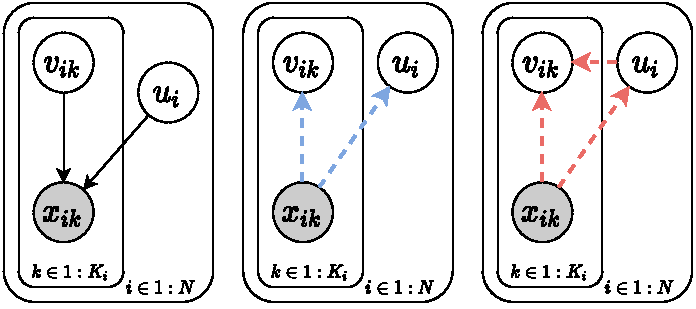
\includegraphics[width=\columnwidth]{files/pgm.pdf}}
    \caption{Group-instance generative model (\textbf{left}). Variational latent posterior of current methods (\textbf{middle}). Our conditional variational latent posterior (\textbf{right}).}
    \label{fig:pgm}
    \end{center}
    \vskip -0.2in
\end{figure}

The current state-of-the-art in GID uses a hierarchical process to model the data: an unobserved group variable $u$ and an independent unobserved instance variable $v_k$ come together to generate an observation $x_k$ \citep{Bouchacourt2018MultiLevelVA, Hosoya2019GroupbasedLO, Nmeth2020AdversarialDW}. This is the group-instance generative model (\cref{fig:pgm}-left). Part of the standard setup is to train this model using the Variational Autoencoder framework \citep{Kingma2014AutoEncodingVB, JimenezRezende2014StochasticBA} by optimising a lower-bound to the data likelihood expressed in terms of a variational latent posterior distribution $q(u, \mathbf{v} | \mathbf{x})$. 

When defining the variational latent posterior,  existing works \citep{Bouchacourt2018MultiLevelVA, Hosoya2019GroupbasedLO, Nmeth2020AdversarialDW, Chen2020WeaklySD} make the simplifying assumption that the group and instance variables are conditionally independent given the observations (\cref{fig:pgm}-middle).  We refer to this property as the \textit{independence assumption}:

\begin{equation}
\label{eq:indep}
q(u, \mathbf{v} | \mathbf{x}) = q(u | \mathbf{x}) \sum_k q(v_k | x_k)
\end{equation}

Our study shows empirically that this assumption hinders disentanglement on a yet unexplored class of downstream problems for GID: these problems have the property that the conditional distribution between the instance variable and observation $p(v | x)$ changes from group to group, thus making it impractical and even unfeasible to infer the instance variable from a single observation. We call these \textit{group-confounded problems} because the group variable acts as a confounder for the relationship between $x$ and $v$.

Our strategy to learn representations under group-confounding is deceptively simple: condition the inference variable on the previously inferred group variable $q(v_k | x_k, u)$ (\cref{fig:pgm}-right). In statistics, conditioning on the confounding variable is the standard approach to control its effect \citep{Greenland1999ConfoundingAC}.

To our knowledge, we are the first to apply the paradigm of confounding to the group variable in a latent inference problem. GID typically follows the philosophy of fair representations \citep{Louizos2016TheVF, Achille2018EmergenceOI} where the grouping is interpreted as \textit{nuisance variable} whose effect on the inferred instance variable must be minimised using additional regularisation objectives \citep{Nmeth2020AdversarialDW}. As we will show, controlling the effect of the group variable by conditioning on it (confounding approach) rather than training agains it (invariance approach) encourages marginal independence between the latent variables whilst simultaneously allowing for more precision in the estimation of the instance variables.

\subsection{Motivating Problem} 

Consider the problem of multiple imputation in standardized test scores \citep{Gelman2006Data}. We are given a dataset containing the scores of different students over several standardised tests. Some students did not take some tests, so the corresponding scores are missing. The task is to impute the missing scores in order to clean the dataset for further analysis.

Group-instance disentanglement provides a straightforward way to perform multiple imputations on this dataset. First, we establish that the group variable represents the student, and the instance variable represents the test. To impute the score that student $i$ would get on test $j$, we train the GID model on a dataset comprising test scores grouped by students. Second, we infer the instance variables for scores that other students have obtained on test $j$. Finally, we generate a distribution of scores by combining the group variable for student $i$ with the instance variables for test $j$. We can report several statistics of this empirical distribution \citep{Rubin1996MultipleIA} but for our evaluation we take the mean.

On this problem, GID has a considerable advantage over using categorical variables to model tests \citep{Pinheiro2001MixedEffectsMI, Gelman2006Data}: GID can easily generalise to new students and tests without training again \citep{Tenenbaum2000SeparatingSA}. 

The limitation of the current GID methods is the independence assumption \cref{eq:indep}: because the instance variables are inferred separately for each observation the instance encoder discards useful information. Because different students will have different scores for the same test, inferring the test effect without conditioning on the student will produce widely varying estimates across groups \citep{Pinheiro2001MixedEffectsMI}.

In our work, we use this imputation problem as a proof of concept by comparing the existing state-of-the-art in group-instance disentanglement \citep{Bouchacourt2018MultiLevelVA, Hosoya2019GroupbasedLO, Nmeth2020AdversarialDW} with our proposed model, the Context-Aware Variational Autoencoder (CxVAE), that uses a conditional instance encoder. The same conclusions apply to many other similar imputation problems with group-confounding, such as collaborative filtering using matrix factorization models \citep{Koren2009MatrixFT} or imputation in longitudinal studies \citep{Spratt2010StrategiesFM}.

Our contribution is threefold:
\begin{enumerate}
    \item We show empirically that conditioning the instance encoder on the group variable leads to a considerable increase in performance on the multiple imputation task of standardised test scores \citep{Gelman2006Data}. 
    \item Using the Mutual Information Gap \citep{Chen2018IsolatingSO}, we show that the learned representations of the conditional model are more disentangled than the representations of the unconditional models. 
    \item Finally, we investigate the performance gap between our conditional model and the current best unconditional model. We show that this gap can be fully explained by the confounding effect of the group variable, both in terms of multiple imputations error and disentanglement quality.
\end{enumerate}

\section{Background}

The Group-Instance Generative Model \citep{Bouchacourt2018MultiLevelVA,Hosoya2019GroupbasedLO} is a multi-level model that uses two latent variables to generate grouped data: the instance variable $v_{ik} \sim \mathcal{N} (0,1)$ controls the variation within groups, and the group variable $u_i \sim \mathcal{N} (0, 1)$ controls the variation across groups (\cref{fig:pgm}-left). The likelihood of a group $\mathbf{x}$ is:

\begin{equation}
p(\mathbf{x}) = \mathbb{E}_{p(u)}  \prod_{k=1}^{K} \mathbb{E}_{p(v_{k})} ~ [p(x_{k} | u, v_{k})]
\end{equation}

We sometimes omit the index of the group $i$ for simplicity, since the groups are independent and identically distributed.

\subsection{Variational Inference}

Because the exact likelihood is intractable, the standard approach to train the GID model is with a Variational Autoencoder \citep{Kingma2014AutoEncodingVB,JimenezRezende2014StochasticBA} which performs optimisation by introducing a variational latent posterior $q(u, \mathbf{v} | \mathbf{x})$ and maximizing the Evidence Lower Bound \citep{Jordan2004AnIT}:

\begin{equation}
\log p(\mathbf{x}) \geq \mathbb{E}_{q(u, \mathbf{v} | \mathbf{x})} [\log p(\mathbf{x} | u, \mathbf{v})] - \mathrm{KL} [q(u, \mathbf{v} | \mathbf{x}) || p(u, \mathbf{v})]
\end{equation}

Existing methods use a class of variational distributions that assume conditional independence between the latent variables.

\begin{equation}
q(u, \mathbf{v} | \mathbf{x}) = q(u | \mathbf{x}) \prod_{k=1}^K q(v_k | x_k)
\end{equation}

\section{Context-Aware Variational Autoencoder}

We propose a new model which can perform well on group-confounded problems. We call our model the Context-Aware Variational Autoencoder (CxVAE). 

The defining feature of our model is a variational latent posterior whose instance variable is conditioned on the group variable:

\begin{equation}
q(u, \mathbf{v} | \mathbf{x}) = q(u | \mathbf{x}) \prod_{k=1}^K q(v_k | x_k, u)
\end{equation}

Thus, the instance encoder is implemented as a network which takes as input the concatenation of the observation $x_k$ and previously sampled group code $\hat{u}$.

\begin{equation}
q(v_k | x_k, u) = \mathcal{N} (\mu, \sigma), ~ (\mu, \sigma) = f (x_k, u),
\end{equation}

This form of variational latent posterior is likely to learn a disentangled representation because it has the potential to learn the true generative latent posterior, which is disentangled by definition. The generative latent posterior can be factorized as:

\begin{equation}
p(u, \mathbf{v} | \mathbf{x}) = p(u | \mathbf{x}) \prod_{k=1}^K p(v_k | x_k, u)
\end{equation}

Existing methods use $q(v_k | x_k)$ as a proxy for $p(v_k | x_k, u)$, which makes their encoders vulnerable to the confounding effect of the group factor.

We are the first to apply the idea of conditioning the instance variable on the group variable to GID. This idea has been previously used in the related problem of sequence disentanglement \citep{Hsu2017UnsupervisedLO, Li2018DisentangledSA}, another example of a group-confounded problem: the variable controlling the long time-scale confounds the inference of the variable controlling the short time scale.

\section{Evaluation}

We show that by making the instance encoder conditional on the inferred group variable, we obtain a considerable gain in multiple-imputation accuracy and a marked improvement in disentanglement.

\subsection{Dataset}

\begin{figure}[t]
    \vskip 0.2in
    \begin{center}
    \centerline{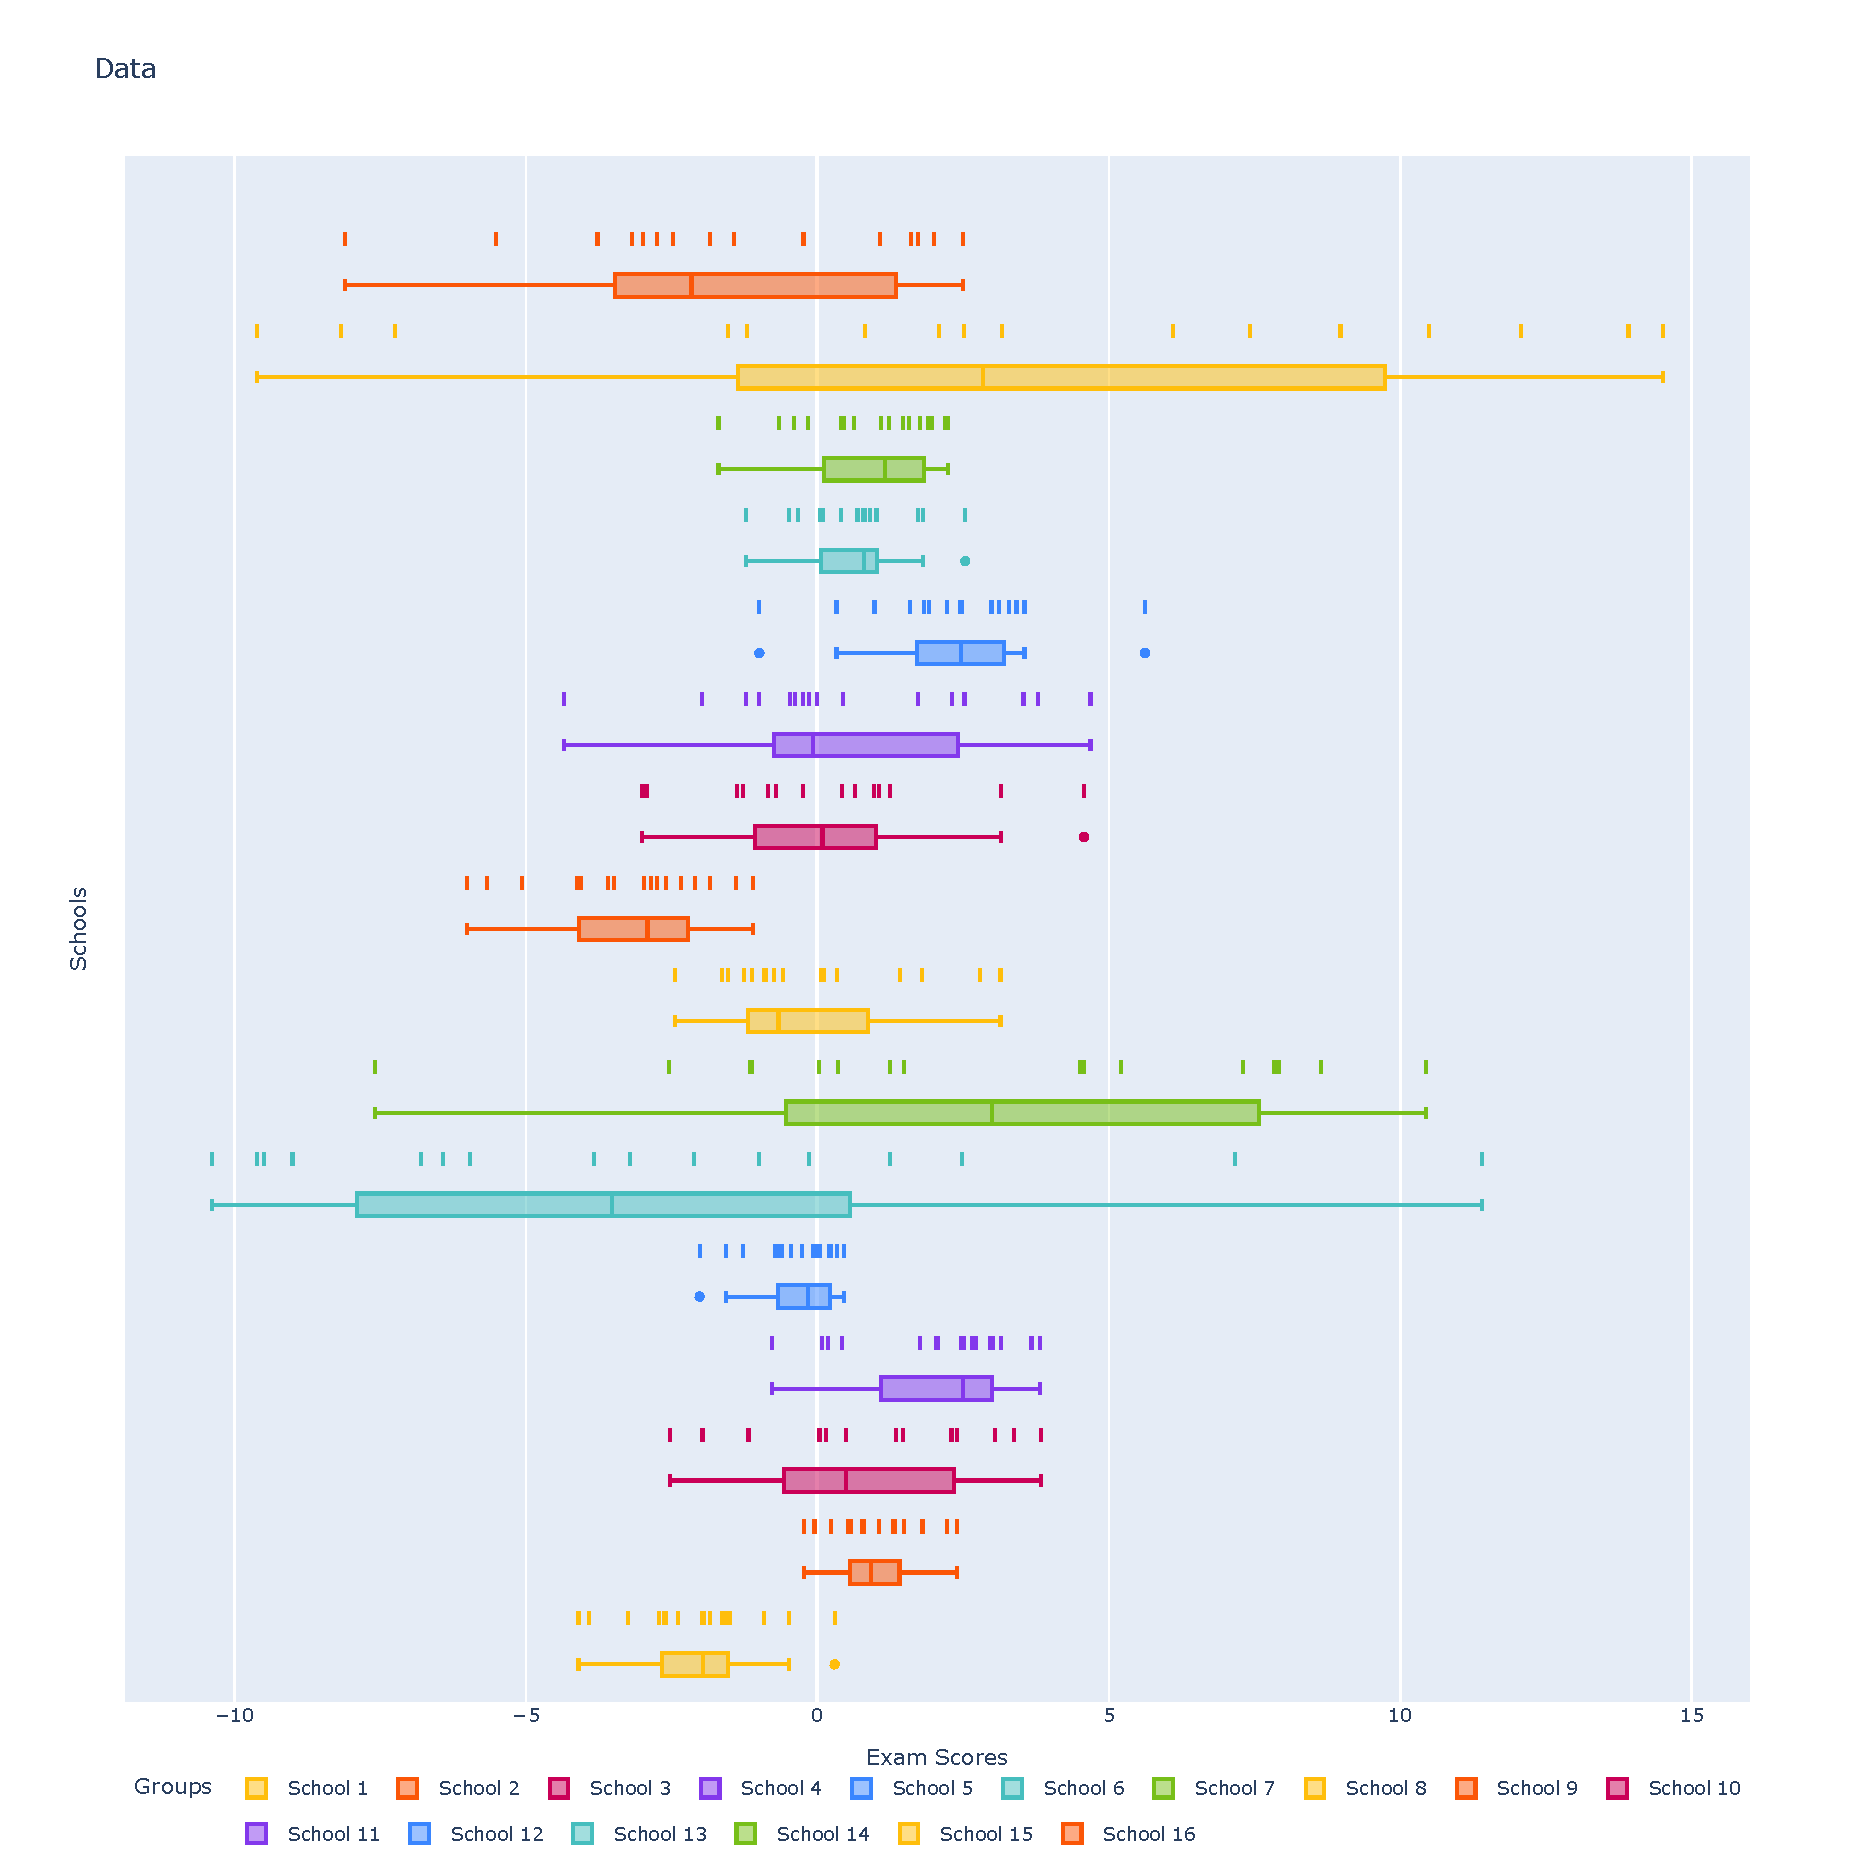
\includegraphics[width=\columnwidth]{files/data.pdf}}
    \caption{\textbf{Dataset with confounding: test scores.} The score of student $i$ on test $j$ is a function of the student's aptitude profile $\alpha_i, \beta_i$ (the group variable) and the test difficulty $\delta_j$ (the instance variable). The green bar shows ``what difficulty test must have student $i$ taken in order to get the score $0.5$''. The test difficulty has markedly different values for different students.}
    \label{fig:data}
    \end{center}
    \vskip -0.2in
\end{figure}

We generate a synthetic dataset with the ``varying intercept, varying slope'' mixed model used in \citet{Gelman2006Data} to model student scores on multiple standardised tests. The score of student $i$ on test $j$ is generated as a function of the student's aptitude profile $\alpha_i, \beta_i$ (the group variablce) and the test difficulty $\delta_j$ (the instance variable). We assume all factors to be normally distributed:

\begin{align} \label{eq:score}
& s_{ij} = 2 \alpha_i - (\beta_i^2 + 1) \delta_j + \epsilon_{ij} \\
& \alpha_i, \beta_i, \delta_j \sim \mathcal{N} (0,1) \\
& \epsilon_{ij} \sim \mathcal{N} (0, 0.1)
\end{align}

A quick look at the dataset generated by this process reveals that the group is a confounding variable (\cref{fig:data}): estimating the instance variable for a particular value of $s_{ij}$ while ignoring the group variable yields large residuals predictive of the group effect.

For the evaluation procedure, we use the above model to generate $N=32,768$ values for $\alpha_i, \beta_i$ and $M=128$ values for $\delta_j$. We then randomly select half of the students and half of the tests to generate a training dataset with $2,097,152$ scores split across $16,384$ groups. We take the other half of students and tests to generate the holdout dataset, so that every testing student and group is unseen at training time. 

Then, we simulate a missing-completely-at-random pattern \citep{Rubin1975InferenceAM} in the training data by removing each score in the dataset with a probability of $0.5$.  We can now build our grouped dataset by re-indexing the remaining training data such that $x_{ik} = s_{ij}$. The number of non-missing scores for student $i$ gives the value of $K_i$.

We use the same exact data-generating model as in \cref{eq:score} as a probabilistic decoder function for the autoencoder models that we evaluate.

We have chosen to evaluate on a synthetic dataset because it allows for fine control over the parameters of the data-generating process (especially relevant in \cref{xy}) and it also enables us to measure the quality of disentanglement using the principled Mutual Information Gap (\cref{mig})

\subsection{Metrics}

We quantitatively evaluate the group-instance disentanglement methods with respect to both multiple imputation performance and quality of disentanglement.

As a general metric, we report the reconstruction error (MSE) on the holdout data for every experiment, commonly used as a proxy for the likelihood of the holdout set.

\subsubsection{Multiple Imputation}

We measure multiple imputation error using the following algorithm:
\begin{enumerate}
\item We split the holdout dataset into 128 batches of 128 students. We pick one student in each batch and randomly remove their scores with probability $0.5$ (we will use these to measure the error). We then use the other 127 students in each batch to predict the missing scores for this student.
\item \textit{How do we predict the missing scores $\mathbf{j}$ of student $a$ with the scores of student $b$?} For student $b$, we infer a set of instance variables from their scores on the same tests as the missing scores of student $a$ by sampling $q(\mathbf{v}_{b, \mathbf{j}} | \mathbf{x}_b)$. For student $a$, we infer the group variable using the non-missing scores by sampling $q(u_a | \mathbf{x}_{a, -\mathbf{j}})$. We then generate the set of missing scores with the group variable of student $a$ and each instance variable of student $b$ by sampling $p(x_{aj} | u_a, v_{aj})$ for every $j \in \mathbf{j}$ missing test.
\item We now have, for each missing score in the holdout dataset, 127 generated scores. We take the squared error between each generated score and the ground-truth missing score, and then average over all generated scores. This is our measure of error.
\end{enumerate}

Multiple imputation in this setting is equivalent to the problem of unsupervised translation in group-instance disentanglement \citep{Tenenbaum2000SeparatingSA}.  In our case, we are translating the scores of student $a$ to the missing scores of student $b$. We can use translation as an additional qualitative comparison between the conditional and unconditional model, which can be seen in \cref{fig:trans}.

\subsubsection{Mutual Information Gap}
\label{mig}

We use the Mutual Information Gap \citep{Chen2018IsolatingSO} to measure the quality of the disentanglement. We measure empirically the amount of mutual information between the inferred latent variables $u,  \mathbf{v}$ and the student effect $\alpha, \beta$ which represents the ground-truth group factor. Consequently, the goal is to have maximum mutual information between the group variable $u$ and the ground-truth, and minimum mutual information between the instance variables $\mathbf{v}$ and the ground-truth.  The gap between the two (normalized with the entropy of the ground-truth factors) is the metric of disentanglement:

\begin{equation}
\mathrm{MIG} = \frac{1}{H(\alpha, \beta)} (I(u; \alpha, \beta) - I(\mathbf{v}; \alpha, \beta))
\end{equation}

Since the data-generating process is known, the mutual information between the inferred group variable and the ground-truth group variable $I(u; \alpha, \beta)$ is straightforward to implement by following the process of \citet{Chen2018IsolatingSO}.

We measure only the mutual information between the ground-truth group factor and the latent variables because,  as pointed out by \citet{Nmeth2020AdversarialDW}, the common failure case we are trying to guard against in group-instance disentanglement is that the instance variables $\mathbf{v}$ might learn information belonging to the ground-truth group factors $\alpha, \beta$.

\subsection{Conditional vs Unconditional Model}

\begin{figure}[t]
    \vskip 0.2in
    \begin{center}
\begin{subfigure}{0.49\columnwidth}
    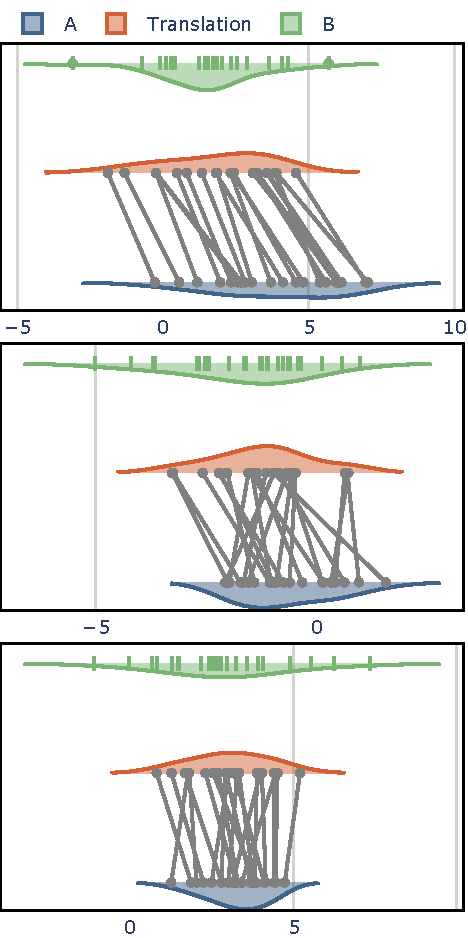
\includegraphics[width=\textwidth]{files/trans_ours.pdf}
    \caption{CxVAE}
\end{subfigure}
\hfill
\begin{subfigure}{0.49\columnwidth}
    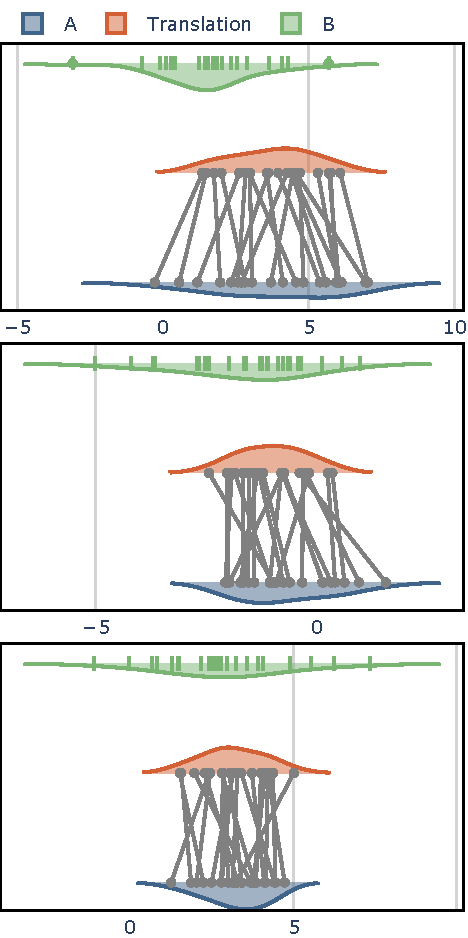
\includegraphics[width=\textwidth]{files/trans_theirs.pdf}
    \caption{GVAE}
\end{subfigure}
    \caption{\textbf{Unsupervised translation with the unconditional GVAE vs our conditional CxVAE}.  The task is to generate a set of test scores (\textbf{middle}) by translating the scores of the source student (\textbf{bottom}) onto the distribution of scores of the target student (\textbf{top}).  Visual inspection suggests that our model better captures the distribution of the target group.}
    \label{fig:trans}
    \end{center}
    \vskip -0.2in
\end{figure}

\begin{figure}[t]
\vskip 0.2in
\begin{center}
\centerline{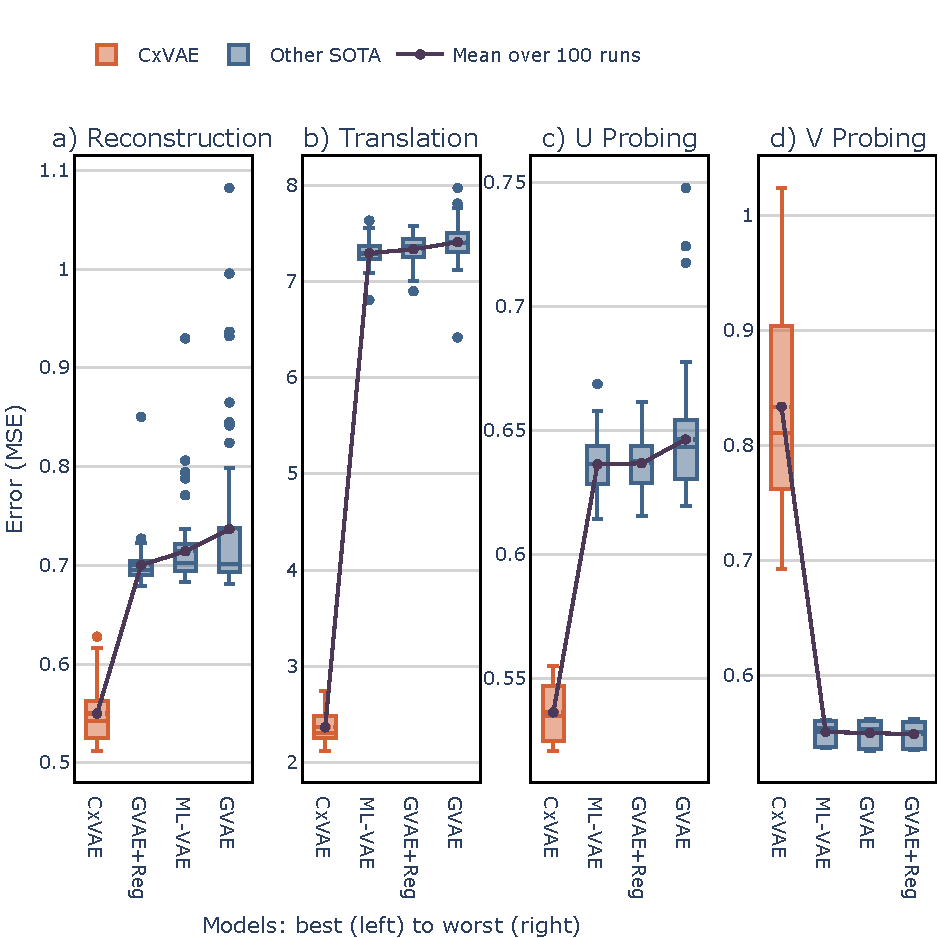
\includegraphics[width=\columnwidth]{files/results.pdf}}
\caption{Our CxVAE produces considerable improvements over the state-of-the-art in every metric considered: holdout reconstruction error (\textbf{lower is better}), multiple imputation error (\textbf{lower is better}), MIG disentanglement score (\textbf{higher is better}).}
\label{fig:results}
\end{center}
\vskip -0.2in
\end{figure}

\begin{figure*}[t]
\vskip 0.2in
\begin{center}
\centerline{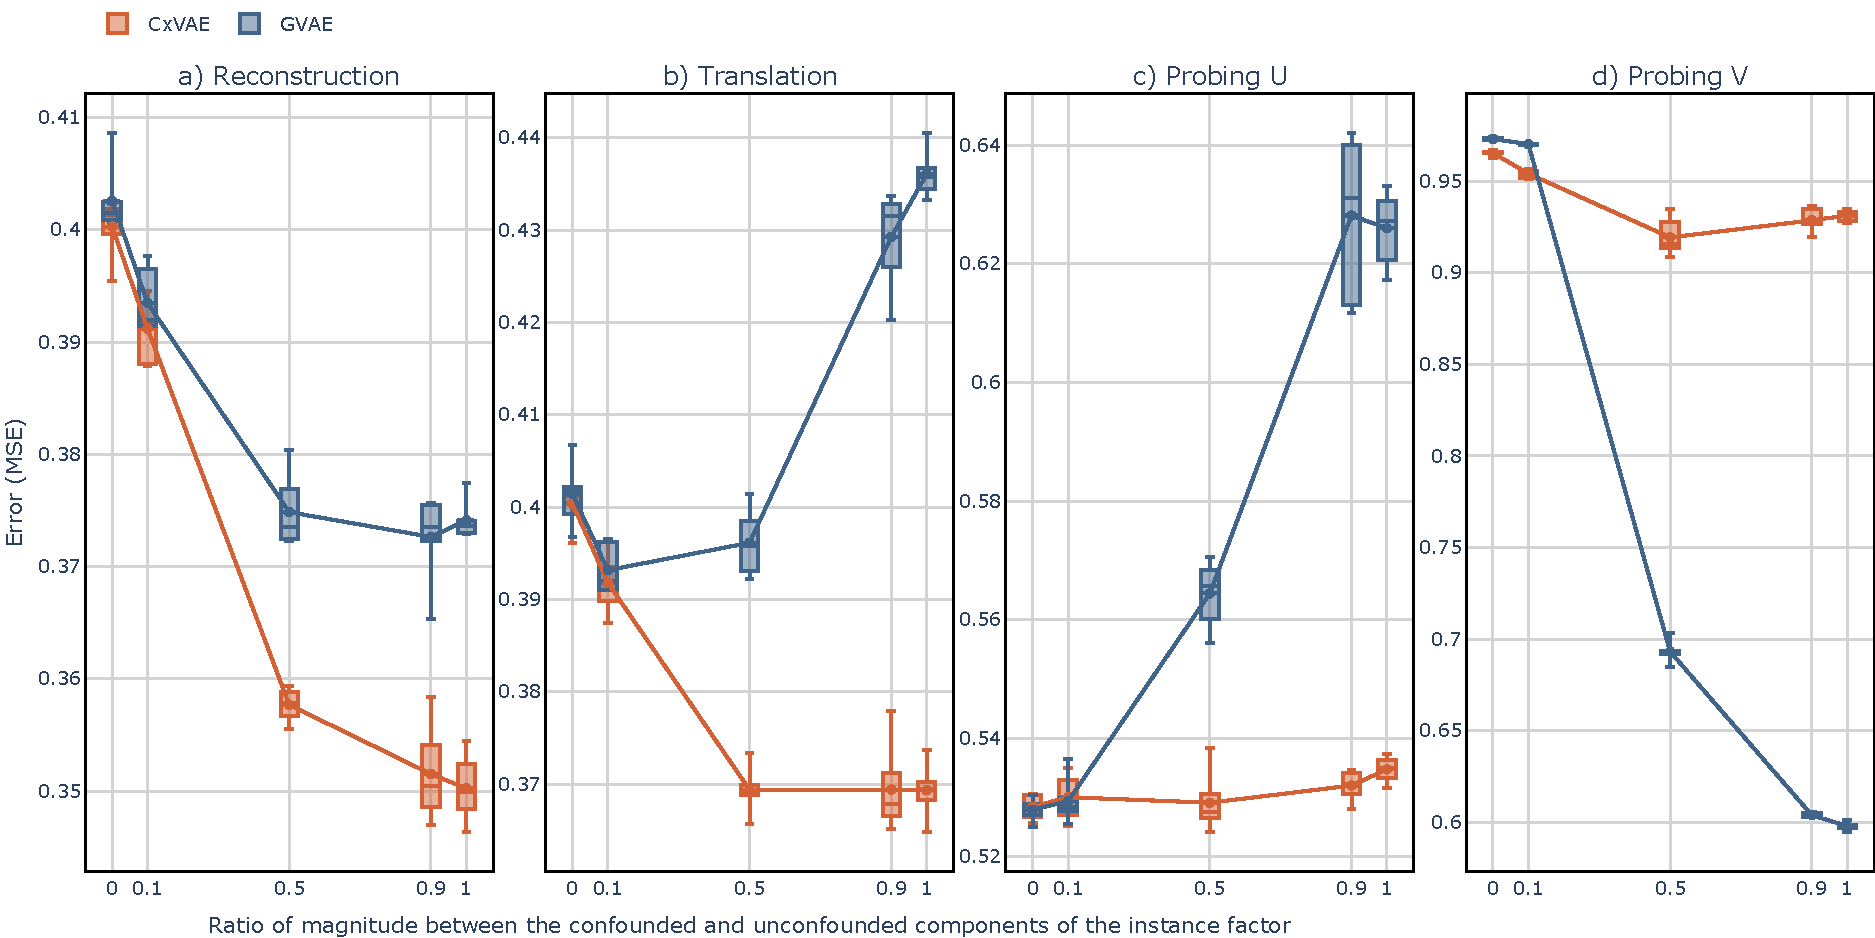
\includegraphics[width=\textwidth]{files/xy_ratio.pdf}}
\caption{\textbf{The performance gain of our CxVAE increases with more confounding.} We show performance on datasets generated with different values of the $\gamma$ hyper-parameter, controlling the strength of the confounding effect. For low values of $\gamma$ the instance factor is not confounded and so the CxVAE and GVAE perform equally well. However, as $\gamma$ increases, GVAE performs more poorly.}
\label{fig:xy}
\end{center}
\vskip -0.2in
\end{figure*}

We compare our conditional CxVAE with the state-of-the-art in group-instance disentanglement, namely the Multi-Level VAE (ML-VAE) \citep{Bouchacourt2018MultiLevelVA}, the Group VAE (GVAE) \citep{Hosoya2019GroupbasedLO} and the Adversarial GVAE (GVAE-AD) \citep{Nmeth2020AdversarialDW}. We implement each encoder as an MLP with 1 hidden layer of 32 activations. The decoder will be the hard-coded generative model from \cref{eq:score}. The group variable will have 2 dimensions (one for $\alpha$ and one for $\beta$) and the instance variable will have 1 dimension (for $\delta$). 

For all experiments, our CxVAE will be a modified GVAE such that the group variable $u_i$ is concatenated with the observation $x_{ik}$ and fed into the instance encoder in order to compute the instance variable $v_{ik}$.

We train each model for 64 epochs, and use the last 10 epochs for evaluation. Additionally, we run the experiment for 100 different random seeds initialisations, both for the data generating process and the networks. We use the same 100 seeds in each model. This gives us 1000 measurements to plot in \cref{fig:results}.

\subsubsection{Results} 

Our CxVAE produces considerable improvements over the state-of-the-art both in terms of multiple imputation accuracy and disentanglement quality (\cref{fig:results}). While the scores of the existing methods cluster together, the gap between them and the CxVAE is larger than the 95\% confidence interval. of any method. Note also that CxVAE produces a smaller reconstruction error on the holdout dataset, suggesting that disentangled representations generalise better to unseen groups.

\section{Strength of Confounding Effect}
\label{xy}

Is the increased performance increase of the our CxVAE due to the fact that the data-generating process is confounded?

To answer this, we modify the data-generating process from \cref{eq:score} by incorporating a hyper-parameter $\gamma$ to control the strength of the confounding effect that the group variable has on the conditional distribution between the instance variable and the data observation $p(v|x)$. For $\gamma=1$, the confounding will be the same as before. For $\gamma=0$, there will be no confounding. Our modified data-generating process is the following:

\begin{align}
& s_{ij} = \begin{bmatrix}
\gamma 2 \alpha_i - (\beta_i^2 + 1)^\gamma \delta_j + \epsilon_{ij}\\
2 \alpha_i - \gamma (\beta_i^2 + 1) \delta_j + \epsilon_{ij}
\end{bmatrix} \\
& \alpha_i, \beta_i, \delta_j \sim \mathcal{N} (0,1) \\
& \epsilon_{ij} \sim \mathcal{N} (0, 0.1)
\end{align}

Firstly, our data is now 2-dimensional. The models for each component is very similar to the model in \cref{eq:score} and both models share the same generative factors $\alpha_i, \beta_i, \delta_j$. The only difference between components is that in one component, $\gamma$ controls the magnitude of the student effect, while in the other, $\gamma$ controls the magnitude of the test effect.

This model is unconfounded when $\gamma=0$ because each ground-truth factor controls a separate component of the data. Inferring the test effect requires only the test component and can ignore the student component. When $\gamma=1$, the dimensions of the data are duplicates, so the problem is exactly the same as previously.

As an intuition, this 2-dimensional model corresponds to a setting where students take a similar practice test before each test, and we suspect that the impact the student-effect has on the score compared to the test-effect changes. Therefore, we assign one dimension of the data to the practice test and one to the actual test, and model the trade-off between effects with the hyper-parameter $\gamma$.

If our hypothesis is correct, that the confounding effect of the group variable causes the performance gap between the conditional and unconditional models, then the gap should decrease as $\gamma$ approaches 0.

\subsubsection{Results} 

The measurements displayed in \cref{fig:xy} confirm our expectations. For low values of $\gamma$ the performance of our CxVAE is evenly matched to the GVAE.  As $\gamma$ increases, CxVAE scores remain relatively stable while GVAE scores decrease substantially.  It is clear that the degree of confounding in the dataset explains the performance gain that we see in the CxVAE. 

\section{Related Work}

\paragraph{Group-Instance Disentanglement} Recent work \citep{Shu2020Weakly, Locatello2020WeaklySupervisedDW} has identified GID as a subproblem of weakly-supervised disentanglement, where disentangled representations are learned with the help of non-datapoint supervision (e.g. grouping, ranking, restricted labelling). Early work in this area focused on separating between visual concepts \citep{Kulkarni2015DeepCI, Reed2015DeepVA}. This area has received renewed interest after the theoretical impossibility result of \citet{Locatello2019ChallengingCA} and the identifiability proofs of \citet{Khemakhem2020VariationalAA} and \citet{Mita2021AnID}. However, a key aspect of recent weakly-supervised models is the interpretation of the grouping as a signal of similarity between datapoints \citep{Chen2020WeaklySD}. 

In our case, we interpret the grouping as a structural factor which enables our model to accumulate evidence from multiple observations even at test-time. This view is clearly present in the related problem of sequence disentanglement \citep{Hsu2017UnsupervisedLO, Denton2017UnsupervisedLO, Li2018DisentangledSA}, where the instance variable (short timescale) is always inferred conditionally on the group variable (long timescale).

\paragraph{Confounding} This concept has been studied since the dawn of statistics and is most rigorously defined in the causal inference literature: confounding is present if an intervention (treatment) on the source variable $x$ changes the conditional distribution of a target variable $p(y | \mathrm{do}(x)) \neq p(y | x)$ \citep{Greenland1999ConfoundingAC}. Usually the confounding variable $u$ is a parent of both source $x$ and target $y$, and the solution is to control for $u$ by conditioning on it or stratifying the experiment. 

The notion of a grouping variable acting as a confounder when learning a predictor also has a long history in the field of supervised learning \citep{Morabia2010HistoryOT}. When the confounder manifests as a distribution shift rather than as discrete groups, this phenomenon also comes under the name of population drift \citep{Kelly1999Impact}, a defining feature of federated learning \citep{Kairouz2021AdvancesAO}.

\section{Conclusions}

In this work, we investigate the problem of group-instance disentanglement in settings where the inference of the instance variable is confounded by the group variable. We show empirically that conditioning the instance encoder on the group variable produces better disentangled representations than the unconditional models that comprise the current state-of-the-art. We also show that the strength of the confounding effect in the dataset determines the performance gap between the conditional and unconditional models. Our evaluation is run on the downstream task of multiple imputation on grouped data, a problem on which group-instance models have not been applied before.

\bibliography{main}
\bibliographystyle{icml2022}


%%%%%%%%%%%%%%%%%%%%%%%%%%%%%%%%%%%%%%%%%%%%%%%%%%%%%%%%%%%%%%%%%%%%%%%%%%%%%%%
%%%%%%%%%%%%%%%%%%%%%%%%%%%%%%%%%%%%%%%%%%%%%%%%%%%%%%%%%%%%%%%%%%%%%%%%%%%%%%%
% APPENDIX
%%%%%%%%%%%%%%%%%%%%%%%%%%%%%%%%%%%%%%%%%%%%%%%%%%%%%%%%%%%%%%%%%%%%%%%%%%%%%%%
%%%%%%%%%%%%%%%%%%%%%%%%%%%%%%%%%%%%%%%%%%%%%%%%%%%%%%%%%%%%%%%%%%%%%%%%%%%%%%%
%%%%%%%%%%%%%%%%%%%%%%%%%%%%%%%%%%%%%%%%%%%%%%%%%%%%%%%%%%%%%%%%%%%%%%%%%%%%%%%
%%%%%%%%%%%%%%%%%%%%%%%%%%%%%%%%%%%%%%%%%%%%%%%%%%%%%%%%%%%%%%%%%%%%%%%%%%%%%%%


\end{document}


% This document was modified from the file originally made available by
% Pat Langley and Andrea Danyluk for ICML-2K. This version was created
% by Iain Murray in 2018, and modified by Alexandre Bouchard in
% 2019 and 2021 and by Csaba Szepesvari, Gang Niu and Sivan Sabato in 2022. 
% Previous contributors include Dan Roy, Lise Getoor and Tobias
% Scheffer, which was slightly modified from the 2010 version by
% Thorsten Joachims & Johannes Fuernkranz, slightly modified from the
% 2009 version by Kiri Wagstaff and Sam Roweis's 2008 version, which is
% slightly modified from Prasad Tadepalli's 2007 version which is a
% lightly changed version of the previous year's version by Andrew
% Moore, which was in turn edited from those of Kristian Kersting and
% Codrina Lauth. Alex Smola contributed to the algorithmic style files.

